%----------------------------------------------------------------------------------------------------------------------

\begin{frame}{Proposed Idea}

\begin{itemize}
\item Partition given shape into sub-shapes
\item Midcurves can be generated for each sub-shape.
\item Such individual Midcurves are joined 
\end{itemize}
\end{frame}

%----------------------------------------------------------------------------------------------------------------------
\begin{frame}{Part I}
\centering \textbf{\Large Decomposition}
\end{frame}


%----------------------------------------------------------------------------------------------------------------------

\begin{frame}{Polygon Decomposition}
\begin{itemize}
\item A polygon is decomposed into convex regions 
\item By dividing at all reflex (concave) vertices.
\item A reflex vertex can only be removed if the diagonal connecting to it is within the range given by extending its neighbouring edges; otherwise, its angle is only reduced.
\item Choice of location-to-connect-to is crucial
\end{itemize}

%Notes: 

\end{frame}

%----------------------------------------------------------------------------------------------------------------------

\begin{frame}{Decomposition Algorithm}
Let $P$ be a simple polygon.  The Partitioning of $P$ is defined by the decomposition of $P$ into partitions of non-overlapping sub-polygons by adding internal {\em diagonals} between vertices  $P_i$ or by adding new (Steiner) vertices on {\em edges} $\overline{P_i P_j}$.

\begin{list}{}{}

\item 
Go through all the vertices of the polygon one by one in counter-clockwise manner. Current vertex is called $P_i$ %&

\raisebox{-.9\height}{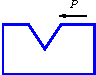
\includegraphics[scale=1.5]{..//Common/images/polydecomp_traverse.pdf} }%\\

%------------------------------------------------------------------------------------------------------------------------------------
\item 
Check if $P_i$ is a Reflex vertex $R$  %&



\raisebox{-.9\height}{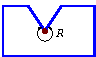
\includegraphics[scale=1.5]{..//Common/images/polydecomp_reflex.pdf} }%\\
\end{list}

\end{frame}

%----------------------------------------------------------------------------------------------------------------------

\begin{frame}{}
\begin{list}{}{}

\item 
Extend lines incident at $P_i$ (the line coming into $P_i$ and going out of $P_i$ ) till they intersect remaining of the Polygon, say at $Q_1$ and $Q_2$. Contour within $Q_1$ and $Q_2$ is called $Range$ %&

\raisebox{-.9\height}{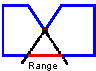
\includegraphics[scale=1.5]{..//Common/images/polydecomp_range.pdf} }%\\

%------------------------------------------------------------------------------------------------------------------------------------
\item 
If there are no $P_i$s within the $Range$ and if any of the $Range$ vertices are close to intersections, separate the triangle out, else, create a new one at the middle on the contour. This newly created point  $Q_m$ is called Steiner point.  $RQ_m$ is the partition-chord to divide the polygon %&

\raisebox{-.9\height}{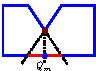
\includegraphics[scale=1.5]{..//Common/images/polydecomp_mid.pdf} }%\\


\end{list}

\end{frame}
%------------------------------------------------------------------------------------------------------------------------------------

\begin{frame}{}
\begin{list}{}{}
\item 
If there are few vertices within the $Range$, choose best one based on following priorities.
\begin{itemize}
\item Highest : Closest Reflex 
\item Medium : Reflex 
\item Low : Closest 
\end{itemize} 
%&

\raisebox{-.9\height}{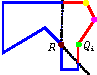
\includegraphics[scale=1.5]{..//Common/images/polydecomp_choice.pdf} }%\\

\end{list}
\end{frame}
%------------------------------------------------------------------------------------------------------------------------------------

\begin{frame}{}
\begin{list}{}{}
\item Once vertex is chosen, say, $Q_i$, create partition chord $RQ_i$ and divide the  polygon.% &
\raisebox{-.9\height}{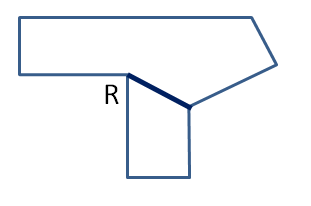
\includegraphics[scale=0.37]{..//Common/images/polydecomp_divide.png} } %\\

\item Send individual sub-polygons to the same process recursively till there are no reflex vertices left. 

\end{list}

\end{frame}
%------------------------------------------------------------------------------------------------------------------------------------

\begin{frame}{Improvements over Bayazit}
Considering even the extreme vertices in the range, thereby giving minimal and elongated partitions. Midcurves are typically for thin-elongated shapes. This improvement results in the sub-polygons of necessary shape characteristics.

\begin{tabular}[h]{@{} p{0.55\linewidth}  p{0.3\linewidth}@{}}

If any of the incoming edges was hitting end points of test line or was collinear, it was getting ignored in the existing algorithm \cite{Bayazit} and then the next closet vertex was getting chosen.   It has been avoided in the improved algorithm. &

\raisebox{-.9\height}{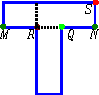
\includegraphics[scale=1.5]{..//Common/images/polydecomp_mine.pdf} }\\

\end{tabular}
\end{frame}

%------------------------------------------------------------------------------------------------------------------------------------

\begin{frame}{Improvements Results}

%\begin{table}[!h]
%\caption{Improvement Over current partitioning algorithm}

\begin{tabular}[h]{@{} p{0.31\linewidth} p{0.31\linewidth} p{0.31\linewidth}@{}}
\toprule

{\bf Shape } & {\bf Bayazit} & {\bf Proposed}\\
\midrule
%------------------------------------------------------------------------------------------------------------------------------------
%T &
\raisebox{0.08\height}{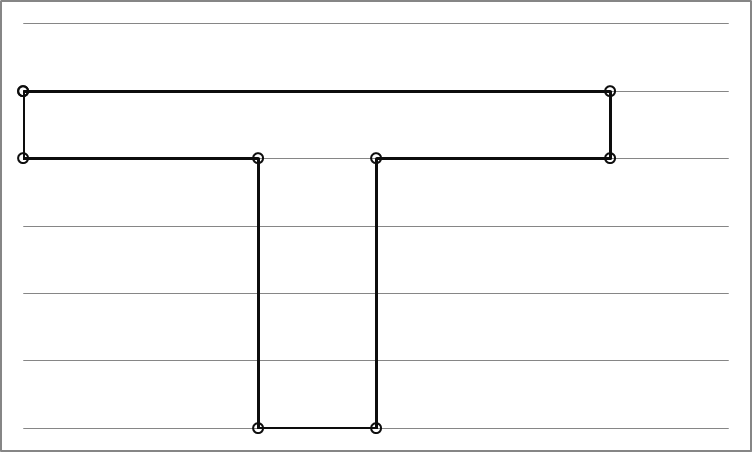
\includegraphics[scale=0.21]{..//Common/images/Ts.png}} &
\raisebox{0.08\height}{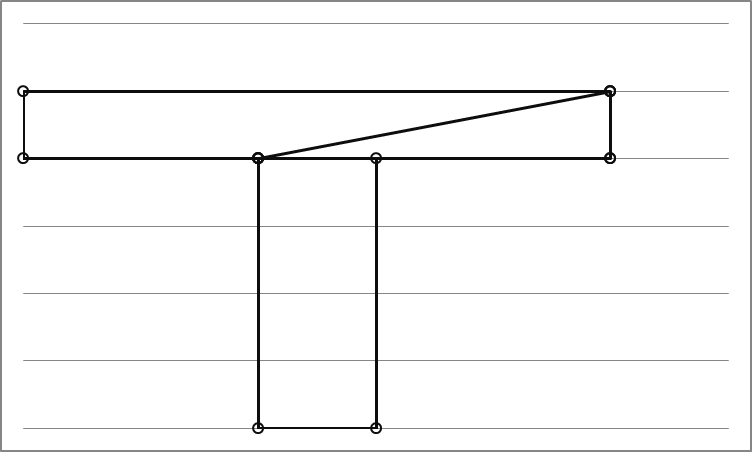
\includegraphics[scale=0.21]{..//Common/images/Tb.png}}&
\raisebox{0.08\height}{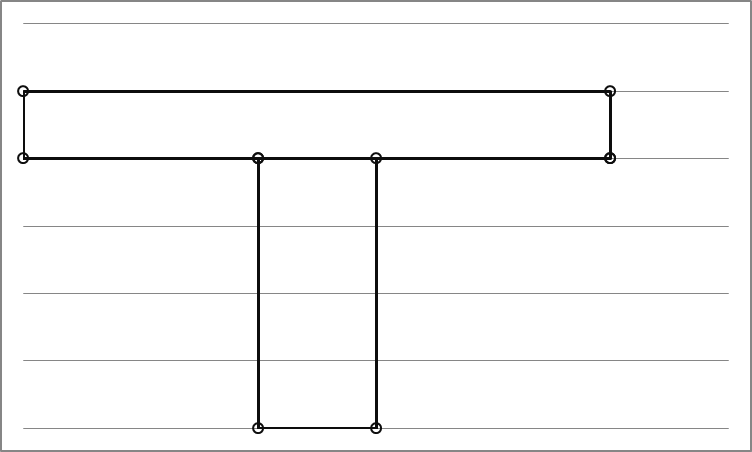
\includegraphics[scale=0.21]{..//Common/images/Tp.png}} \\


%------------------------------------------------------------------------------------------------------------------------------------
%Plus  &
%\raisebox{0.08\height}{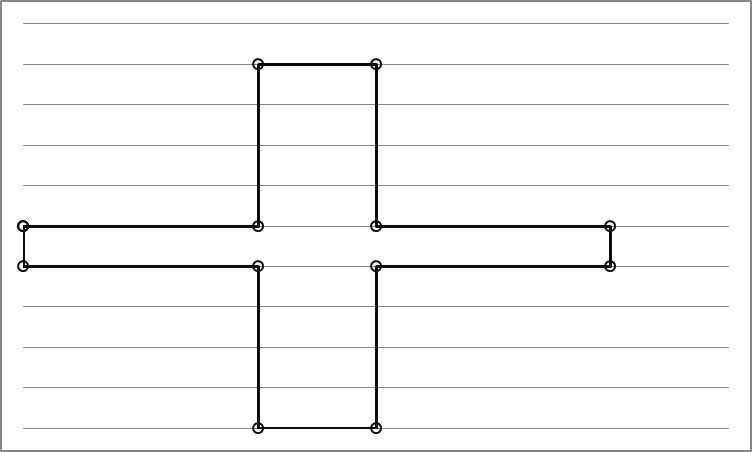
\includegraphics[scale=0.21]{..//Common/images/Pluss.png}} &
%\raisebox{0.08\height}{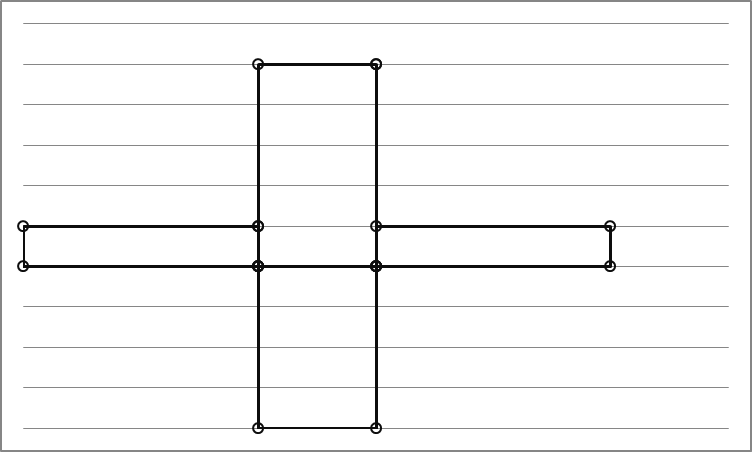
\includegraphics[scale=0.21]{..//Common/images/Plusb.png}}&
%\raisebox{0.08\height}{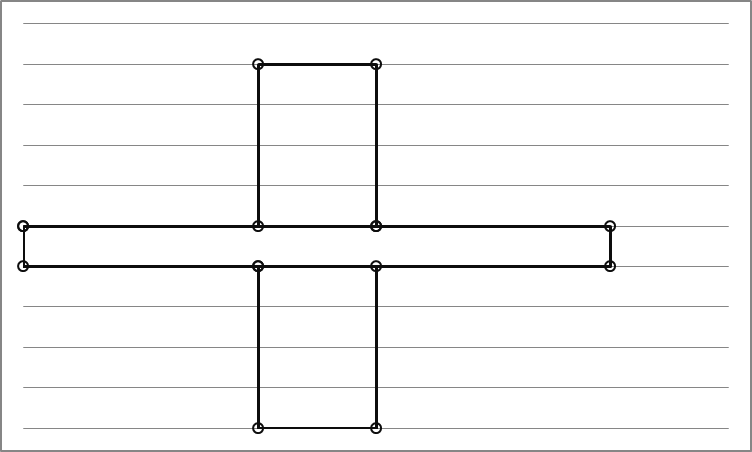
\includegraphics[scale=0.21]{..//Common/images/Plusp.png}} \\


%------------------------------------------------------------------------------------------------------------------------------------
%Star &
\raisebox{0.08\height}{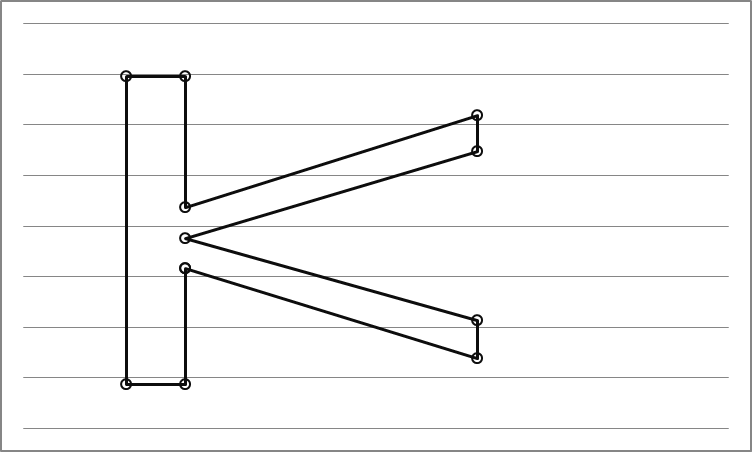
\includegraphics[scale=0.21]{..//Common/images/Ks.png}} &
\raisebox{0.08\height}{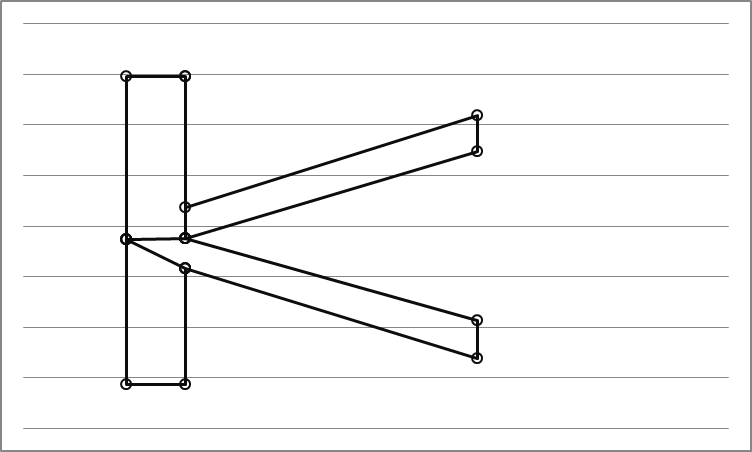
\includegraphics[scale=0.21]{..//Common/images/Kb.png}}&
\raisebox{0.08\height}{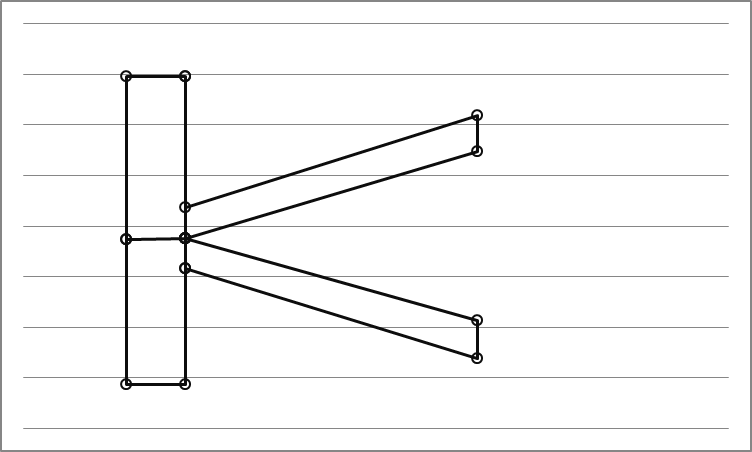
\includegraphics[scale=0.21]{..//Common/images/Kp.png}} \\

%------------------------------------------------------------------------------------------------------------------------------------
%Star &
\raisebox{0.08\height}{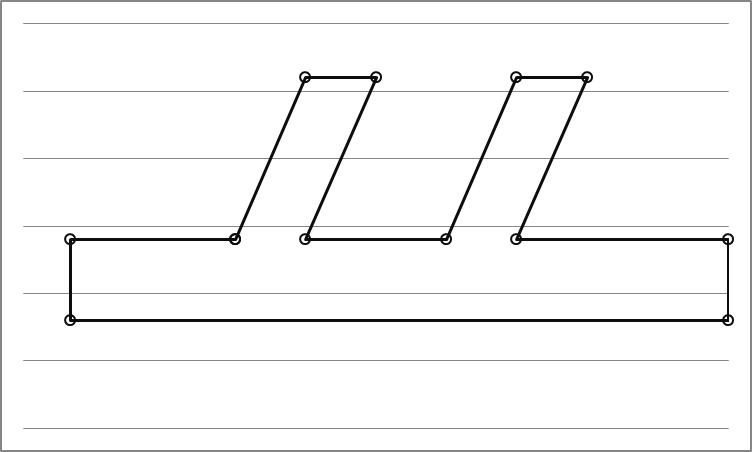
\includegraphics[scale=0.21]{..//Common/images/DoubleKs.png}} &
\raisebox{0.08\height}{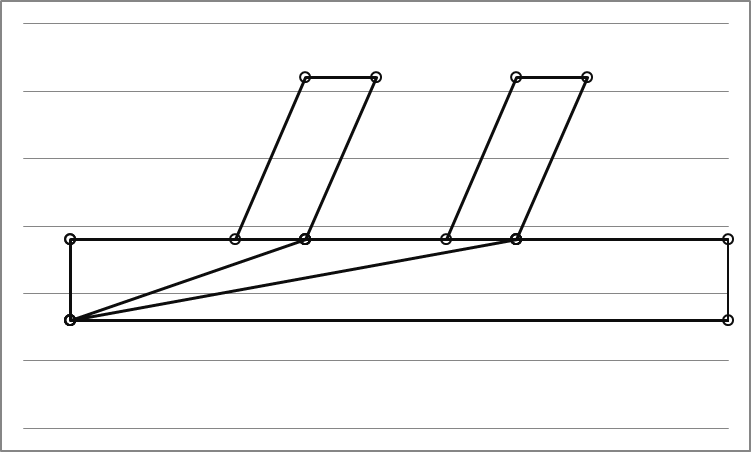
\includegraphics[scale=0.21]{..//Common/images/DoubleKb.png}}&
\raisebox{0.08\height}{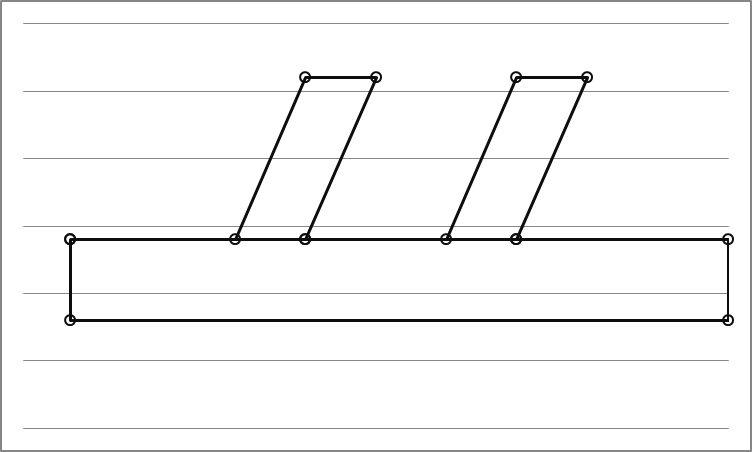
\includegraphics[scale=0.21]{..//Common/images/DoubleKp.png}} \\


\bottomrule
\end{tabular}
%\label{PartitionComparision}
%\end{table}

The resulting sub-polygons are sent for creating midcurves.

\end{frame}
%------------------------------------------------------------------------------------------------------------------------------------

\begin{frame}{Part II}
\centering \textbf{\Large Midcurves}
\end{frame}
%------------------------------------------------------------------------------------------------------------------------------------

\begin{frame}{Midcurve Generation}
\begin{tabular}[h]{@{}p{0.6\linewidth} p{0.3\linewidth}@{}}

Partitioning: Decompose Polygons into  sub-polygons of primitive shapes. Each additional edge inserted during the decomposition is called as 'chord'. &

\raisebox{-.9\height}{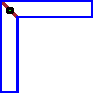
\includegraphics[scale=1.1]{..//Common/images/midcurve_polydecomp.pdf} }\\


%------------------------------------------------------------------------------------------------------------------------------------
Generate Midcurves for individual polygons taking chords into consideration. Midcurves are generated along longer-length and not across shorter width. &
\raisebox{-.9\height}{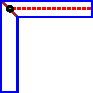
\includegraphics[scale=1.1]{..//Common/images/midcurve_polymid.pdf} }\\


%------------------------------------------------------------------------------------------------------------------------------------
In shapes like 'L' midcurves from both sub-polygons, across the chord, join together at a point, naturally. But in case of shapes like 'T', the horizontal midcurve does not connect , so, needs to be extended to join the other. &

\raisebox{-.9\height}{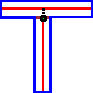
\includegraphics[scale=1.1]{..//Common/images/midcurve_extend.pdf} }\\

\end{tabular}

\end{frame}
%------------------------------------------------------------------------------------------------------------------------------------
